The figure below summarizes the process that was used to answer the research questions.

\begin{figure}[h]
    \centering
    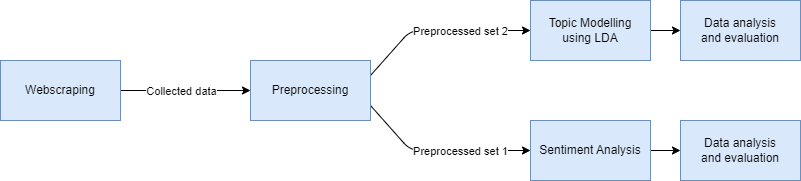
\includegraphics[width=0.8\textwidth]{resources/methodology.png}
    \caption{Summary of the methodology}
    \label{fig:methodology}
\end{figure}

The methodology can be divided into four steps: data collection via webscraping, the preprocessing of the collected data, the processing of the preprocessed data and the analysis along with the evaluation of the analysis. The preprocessing step differs for two analyses. The processing step is further divided into two steps: topic modeling and sentiment analysis. The following sections will discuss each step in detail.